\documentclass[twocolumn,a4j]{jsarticle}
\setlength{\topmargin}{-20.4cm}
\setlength{\oddsidemargin}{-10.4mm}
\setlength{\evensidemargin}{-10.4mm}
\setlength{\textwidth}{18cm}
\setlength{\textheight}{26cm}

\usepackage[top=15truemm,bottom=25truemm,left=15truemm,right=15truemm]{geometry}
\usepackage[latin1]{inputenc}
\usepackage{amsmath}
\usepackage{amsfonts}
\usepackage{amssymb}
\usepackage[dvipdfmx]{graphicx}
\usepackage[dvipdfmx]{color}
\usepackage{listings}
\usepackage{listings,jvlisting}
\usepackage{geometry}
\usepackage{framed}
\usepackage{color}
\usepackage[dvipdfmx]{hyperref}
\usepackage{ascmac}
\usepackage{enumerate}
\usepackage{tabularx}
\usepackage{cancel}
\usepackage{scalefnt}

\renewcommand{\figurename}{Fig.}
\renewcommand{\tablename}{Table }

\lstset{
basicstyle={\ttfamily},
identifierstyle={\small},
commentstyle={\smallitshape},
keywordstyle={\small\bfseries},
ndkeywordstyle={\small},
stringstyle={\small\ttfamily},
frame={tb},
breaklines=true,
columns=[l]{fullflexible},
xrightmargin=0zw,
xleftmargin=3zw,
numberstyle={\scriptsize},
stepnumber=1,
numbersep=1zw,
lineskip=-0.5ex
}

\makeatletter
\def\@maketitle
{
\begin{center}
{\LARGE \@title \par}
\end{center}
\begin{flushright}
{\large 報告書 NO.08 - 2\quad\@date\quad\@author}
\end{flushright}
\par\vskip 1.5em
}
\makeatother

\setcounter{tocdepth}{3}

\author{来代 勝胤}
\title{令和3年度 12月 第3週 報告書}
\date{2021/12/17}

\begin{document}
\columnseprule=0.1mm

\maketitle
\section*{報告内容}
\begin{enumerate}[1.]
    \item 進捗状況
    \item 模擬実験結果
\end{enumerate}

\section{進捗状況}
今週は,引き続き模擬実験を行った。
また,その実験結果のデータ処理を行った。

\section{模擬実験結果}
今後実験を行うにあたり,その手順を明確に決定しておく必要がある.
大量のデータを一度にプログラムで処理できるようにするため,
測定手順を以下のように定めた.\\

\subsection{実験条件}
想定している実験は以下の図の通りである.
\begin{table}[htbp]
    \begin{center}
        \begin{tabular}{|p{30mm}|p{20mm}|p{30}|}
            \hline
            \multicolumn{1}{|c|}{\textgt{条件}} & \multicolumn{1}{|c|}{\textgt{条件数}} & \multicolumn{1}{|c|}{\textgt{条件数}}\\ \hline
            \multicolumn{1}{|c|}{試験片}                    & \multicolumn{1}{|c|}{3} & \multicolumn{1}{|c|}{\textgt{円筒・円柱・角柱}}  \\ \hline
            \multicolumn{1}{|c|}{測定角度}                    & \multicolumn{1}{|c|}{24} & \multicolumn{1}{|c|}{\textgt{15度ごとの測定}}  \\ \hline
            \multicolumn{1}{|c|}{試行回数}                    & \multicolumn{1}{|c|}{$x$} & \multicolumn{1}{|c|}{\textgt{検討中}}  \\ \hline
        \end{tabular}
    \end{center}
\end{table}

\subsection{測定方法}
\begin{itemize}
    \item サンプリング周期は5[Hz]とする
    \item ロードセルをマイクロステージを用いて\\0.03 [mm] ずつ移動させ測定する
\end{itemize}

\subsection{測定準備}
\begin{screen}
    \begin{enumerate}[(1)]
        \item ロードセルを測定する角度に固定
        \item 粗動用ダイヤルでロードセルを大まかな位置に設定
        \item マイクロステージを動かしてロードセルが供試体に接触する位置を0.01[mm]単位で特定
        \item その位置を基準に測定を開始する
    \end{enumerate}
\end{screen}

\subsection{測定手順}
\begin{screen}
    \begin{enumerate}[(1)]
        \item 測定開始から30秒間待機する
        \item 40秒間の測定時間
        \item 30秒間のマイクロステージ操作時間
        \item (2),(3)の作業を5回繰り返す (70秒周期)\\
              ※ 5回目はロードセル,供試体を非接触状態にする
    \end{enumerate}
\end{screen}

\section{実験結果}
今回は,0~90度まで模擬実験を行った.
0度についての結果を以下のFig.1,Fig.2に示す.

\begin{figure}[htbp]
    \footnotesize
    \begin{center}
        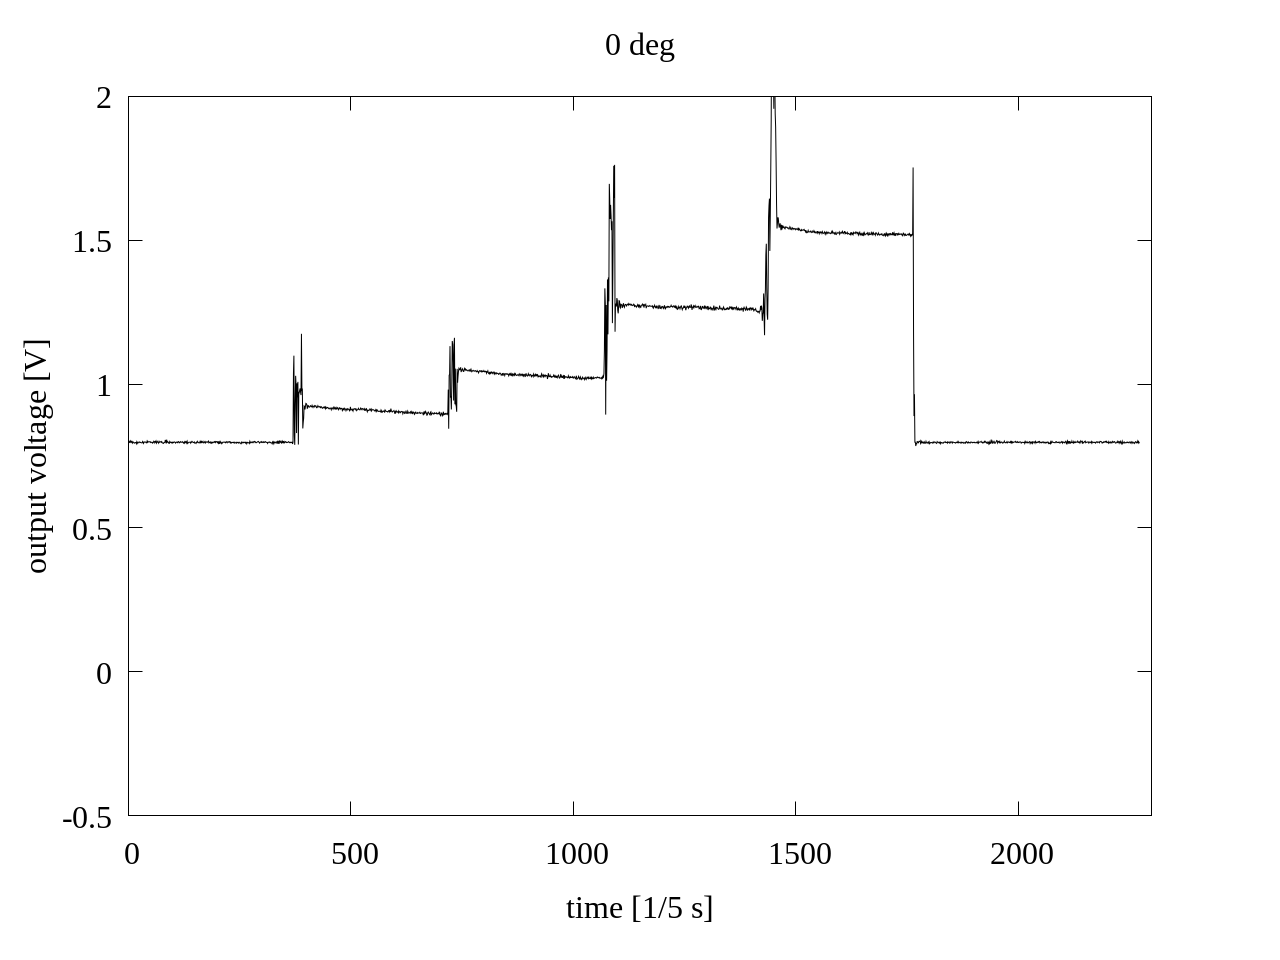
\includegraphics[width=85mm]{../images/reverse/0_loadcell.png}
        \caption{Result of loadcell voltage}
        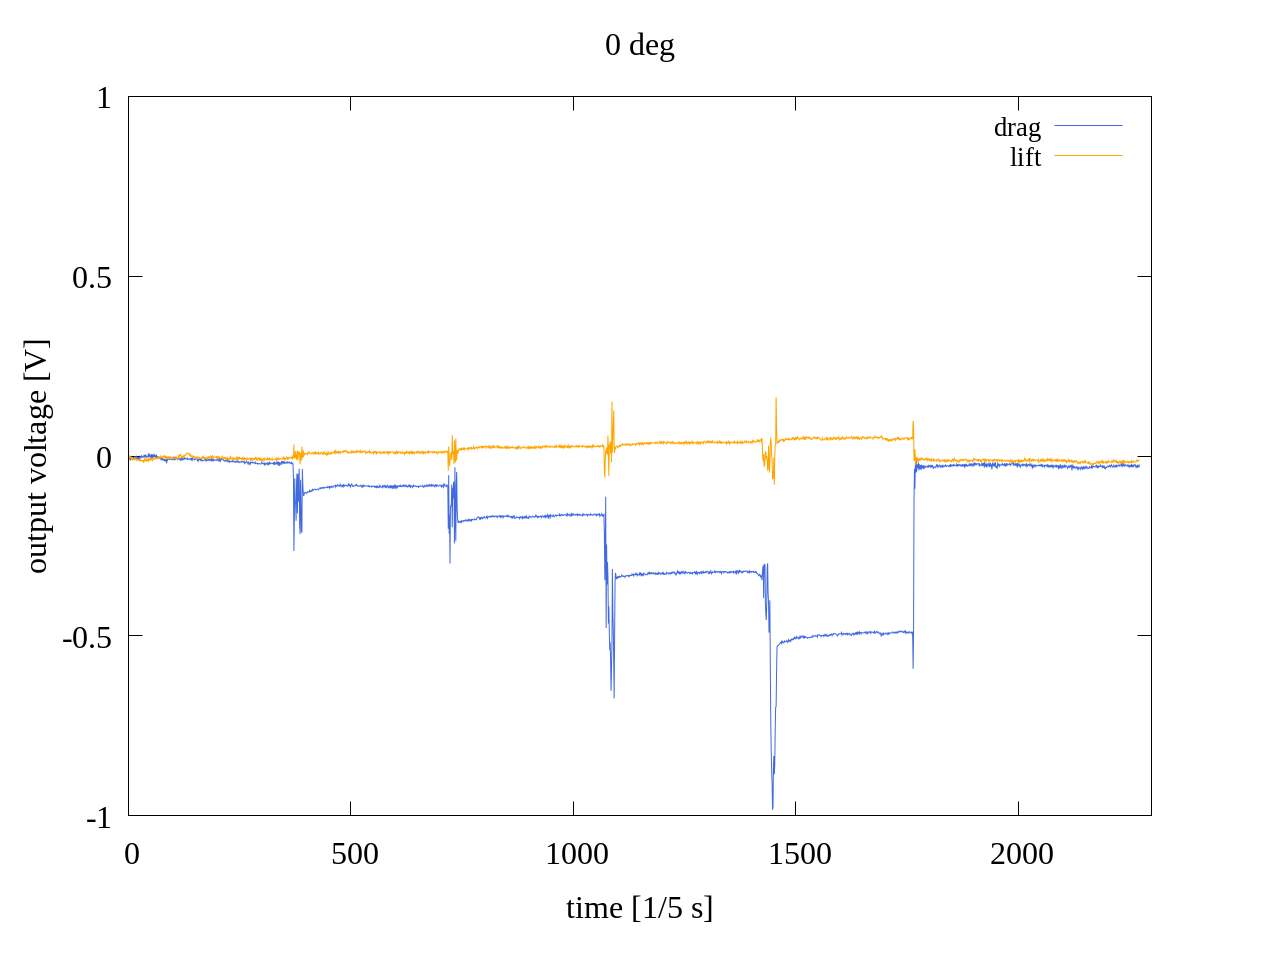
\includegraphics[width=85mm]{../images/reverse/0_strainsensor.png}
        \caption{Result of strainsensor voltage}
    \end{center}
\end{figure}

\section{処理プログラム}
模擬実験から得たデータを用いて,処理プログラムが有効かどうかの検証を行った.

\subsection{ドリフト補正}
以前,作用力測定の実験データ解析に用いたアルゴリズムをもとに
ドリフト補正プログラムを作成し,結果に適用した.
0度についての結果を以下のFig.3~Fig.5に示す.

\begin{figure}[htbp]
    \footnotesize
    \begin{center}
        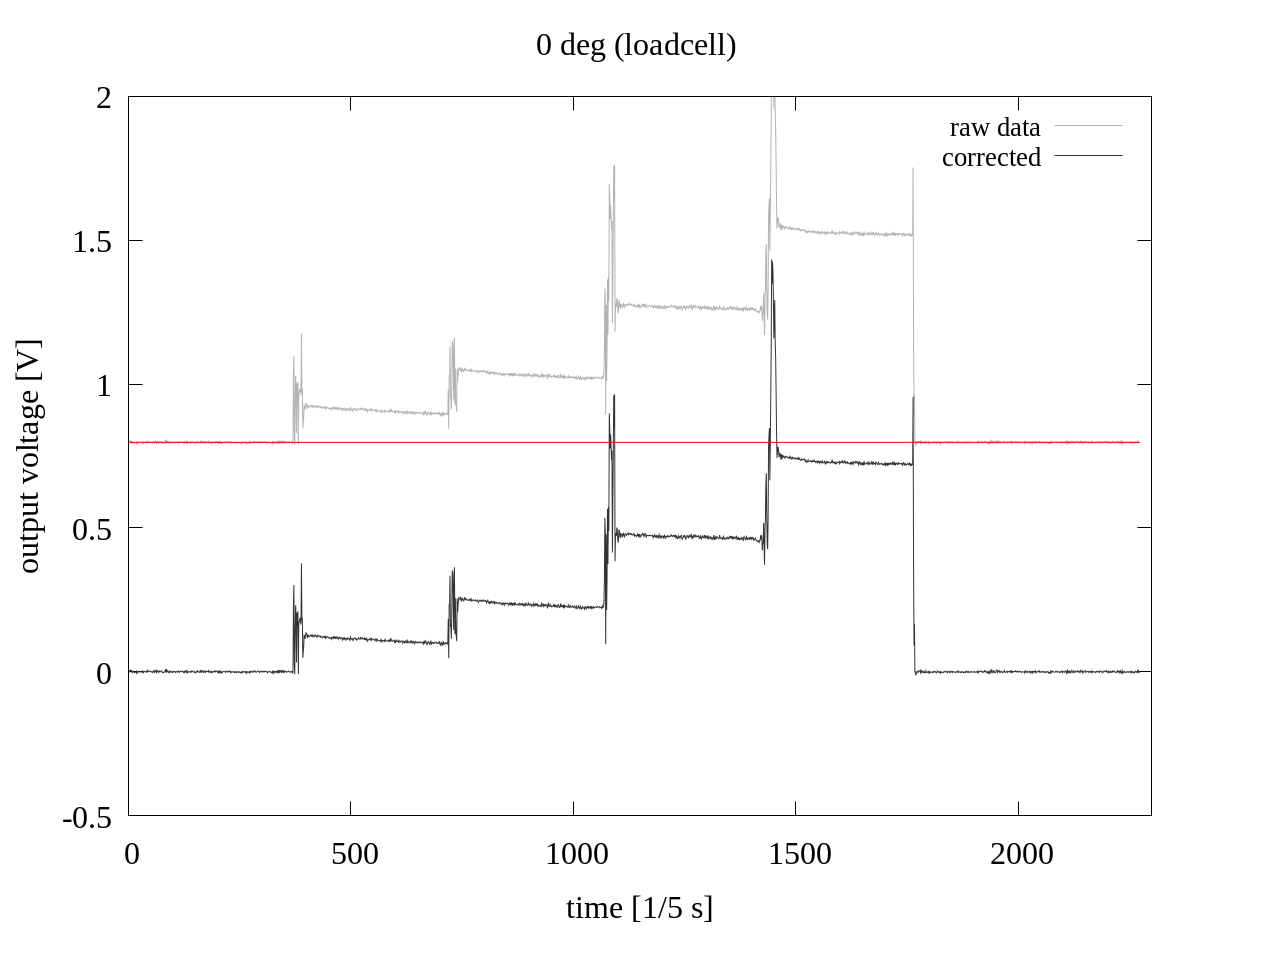
\includegraphics[width=78mm]{../images/drift/0_loadcell_drift.png}
        \caption{Drift correction (loadcell)}
        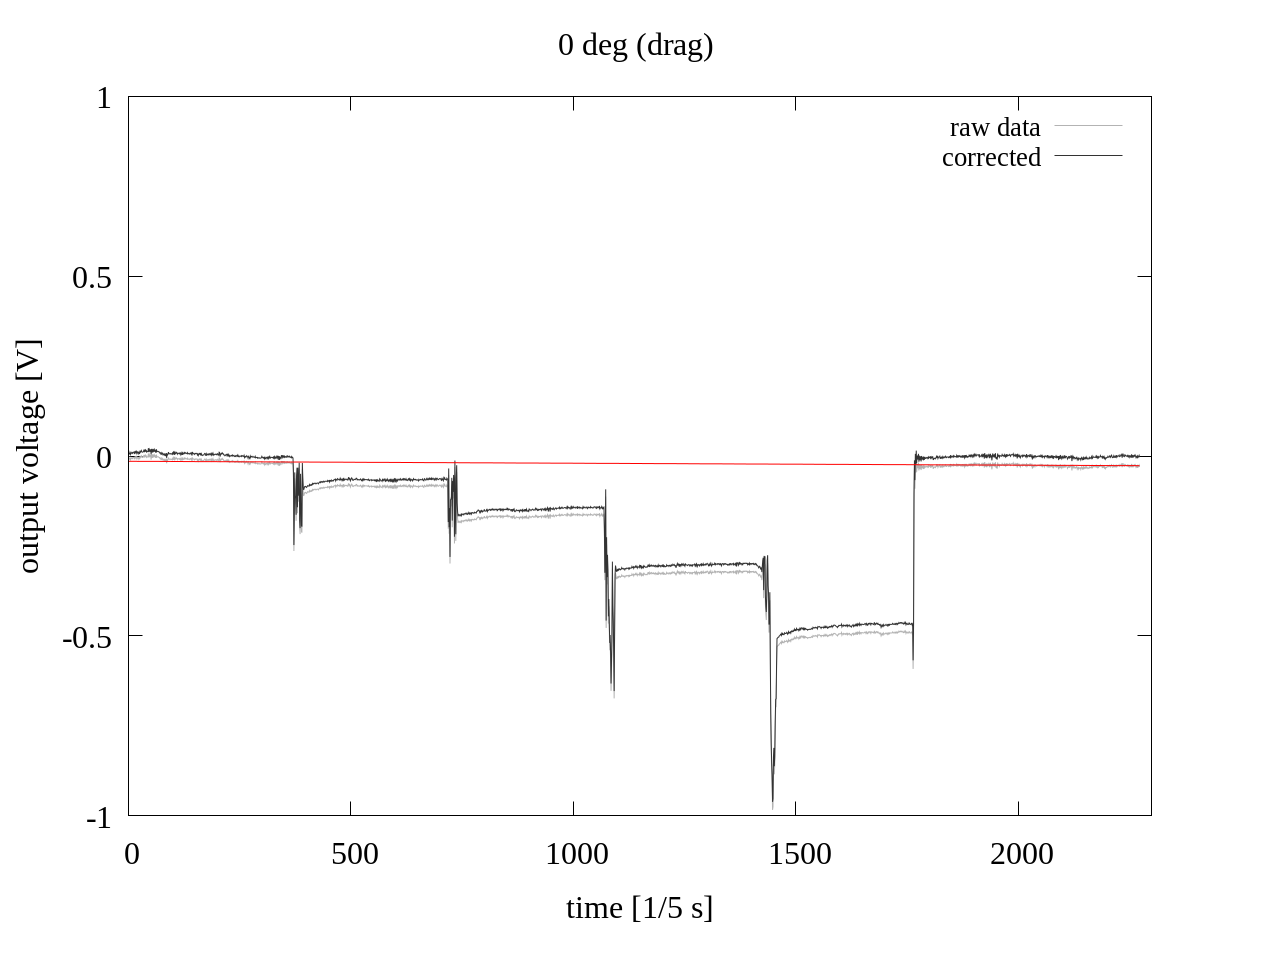
\includegraphics[width=78mm]{../images/drift/0_drag_drift.png}
        \caption{Drift correction (drag)}
        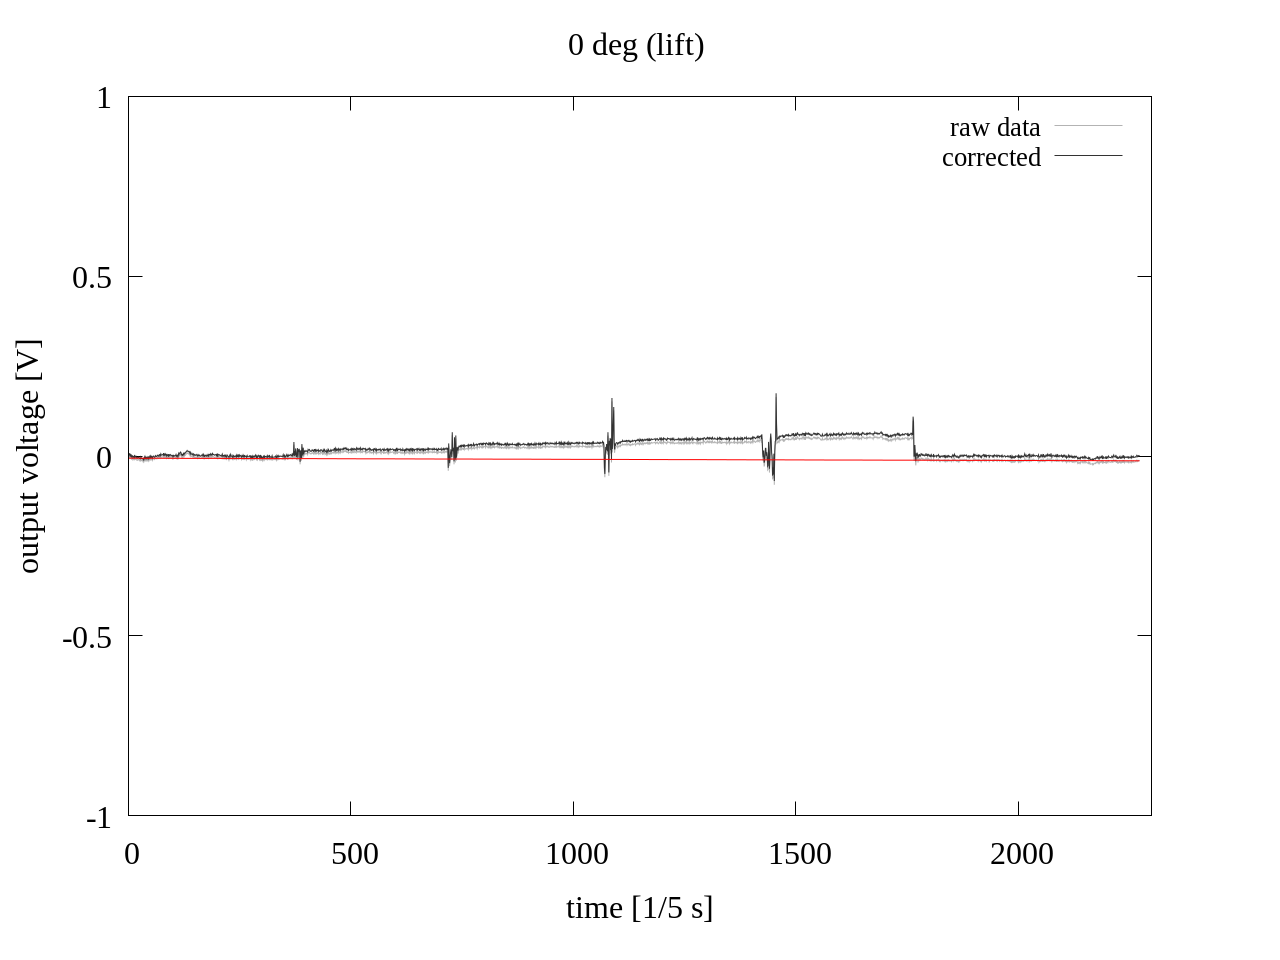
\includegraphics[width=78mm]{../images/drift/0_lift_drift.png}
        \caption{Drift correction (lift)}
    \end{center}
\end{figure}

\newpage

\subsection{平均値の算出}

ドリフト補正を適用した結果を用いて,平均値の結果を算出した.
0度についての結果を以下のFig.6~Fig.8に示す.

\begin{figure}[htbp]
    \footnotesize
    \begin{center}
        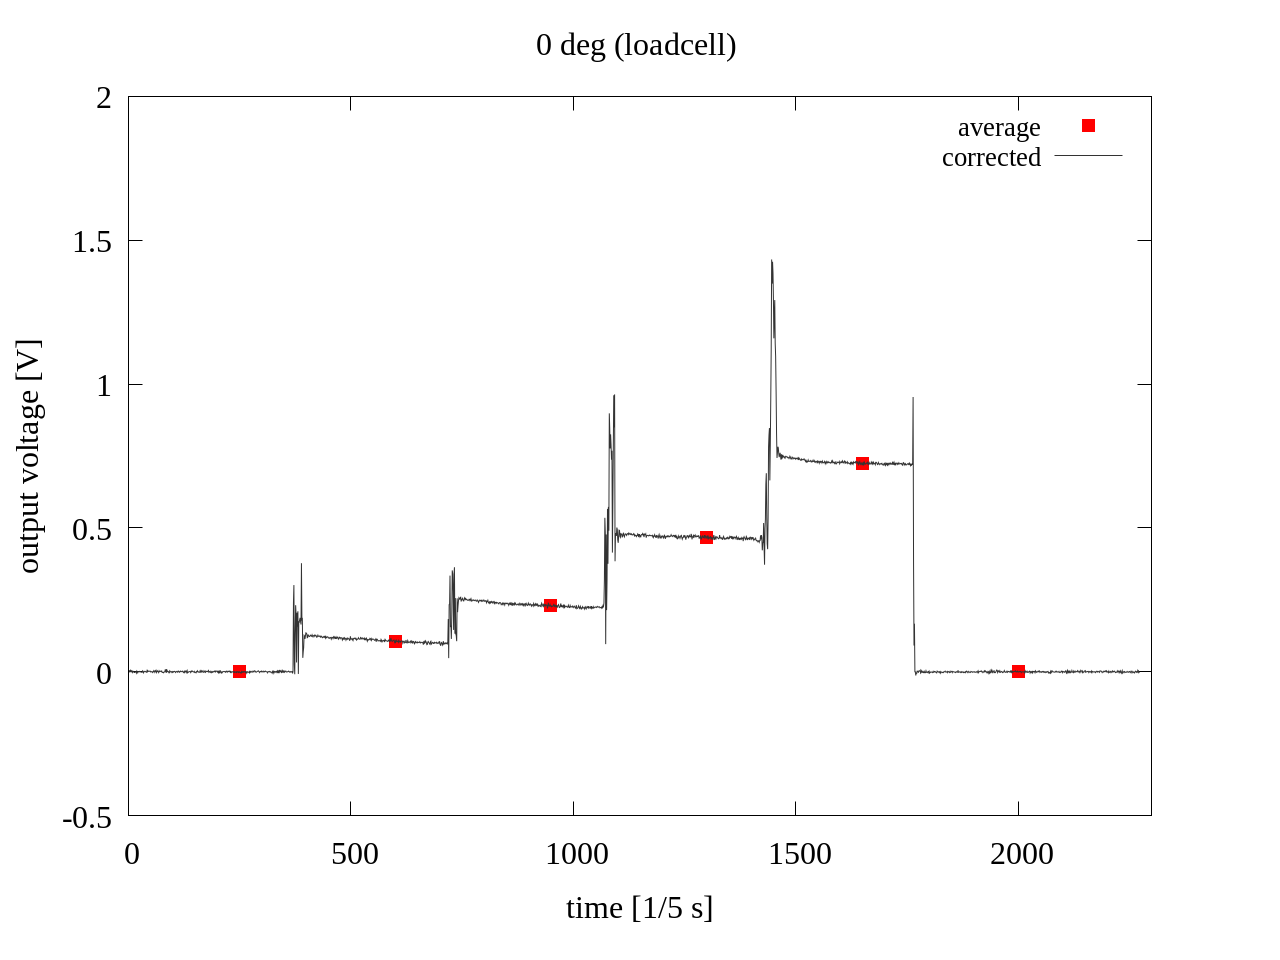
\includegraphics[width=78mm]{../images/average/0_loadcell_average.png}
        \caption{Average calculation (loadcell)}
        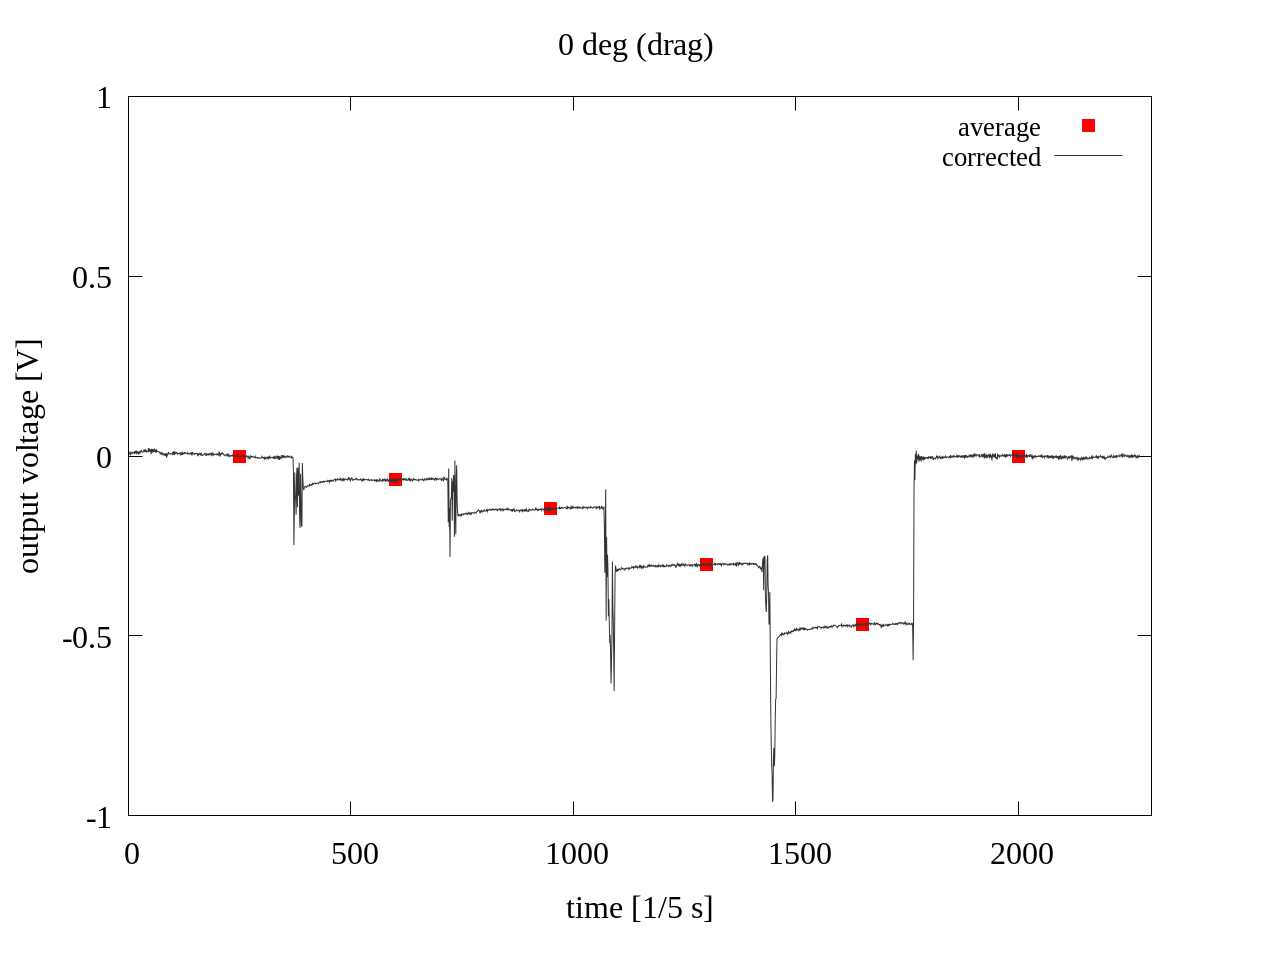
\includegraphics[width=78mm]{../images/average/0_drag_average.png}
        \caption{Average calculation (drag)}
        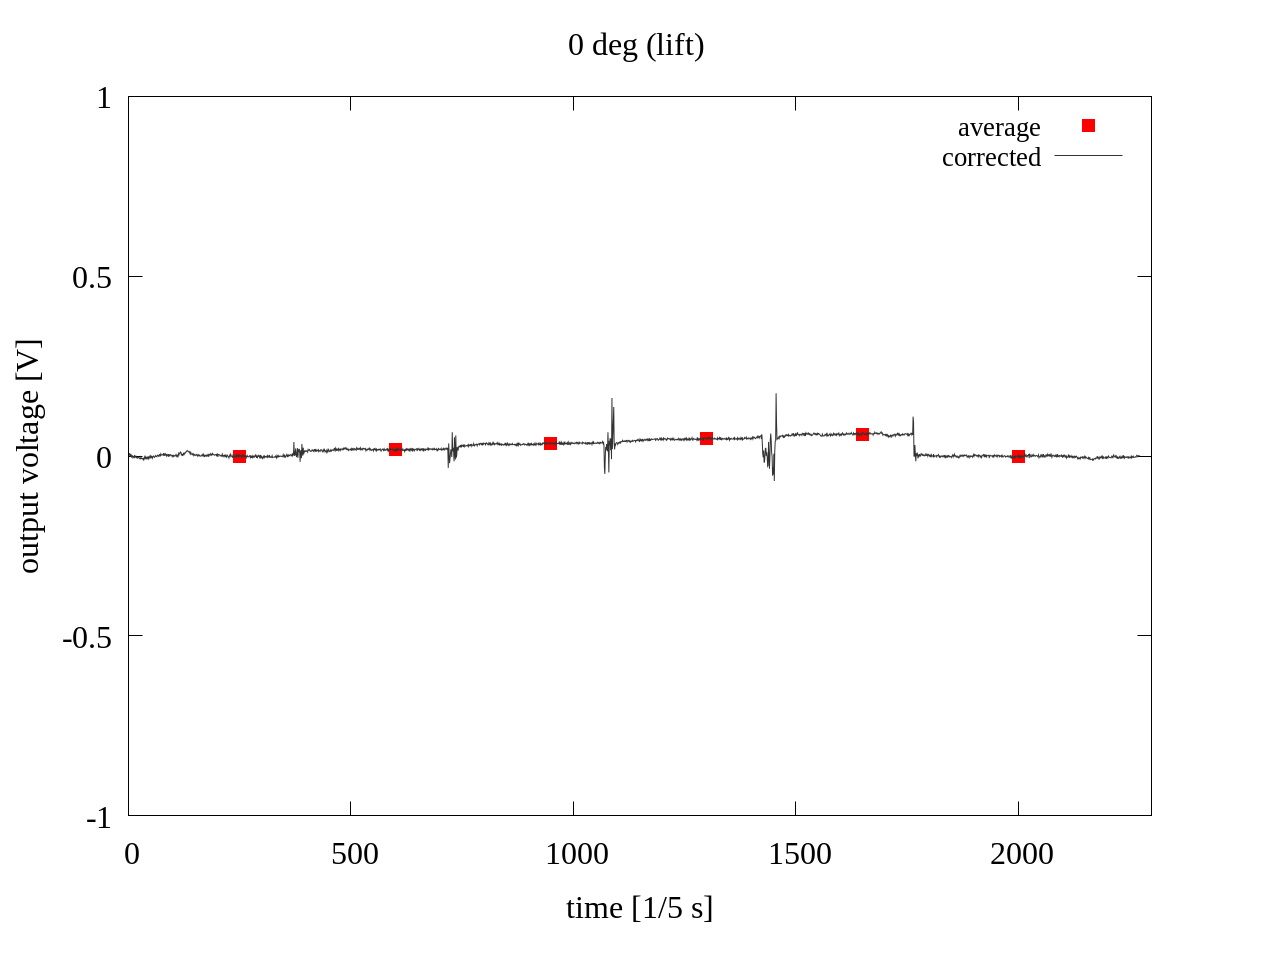
\includegraphics[width=78mm]{../images/average/0_lift_average.png}
        \caption{Average calculation (lift)}
    \end{center}
\end{figure}
\newpage

\subsection{近似直線の算出}
それぞれの出力電圧の平均値を用いて
ロードセルとひずみセンサの関係性について,
最小二乗法を用いて近似直線を算出した.
各角度についての結果を以下のFig.9~Fig.15 に示す.
\begin{figure}[htbp]
    \footnotesize
    \begin{center}
        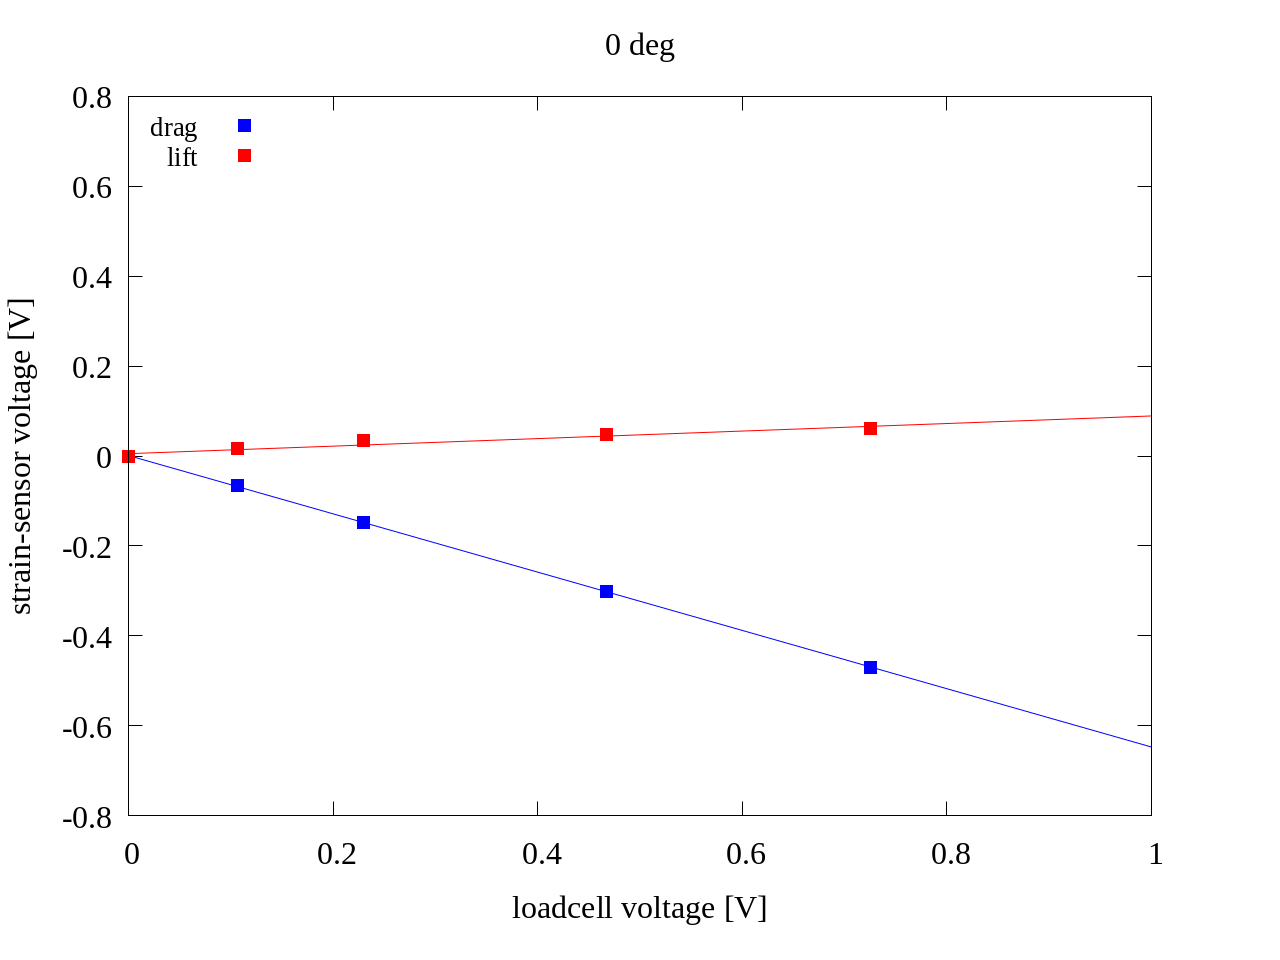
\includegraphics[width=78mm]{../images/linear/0_linear.png}
        \caption{Result of 0 deg}
        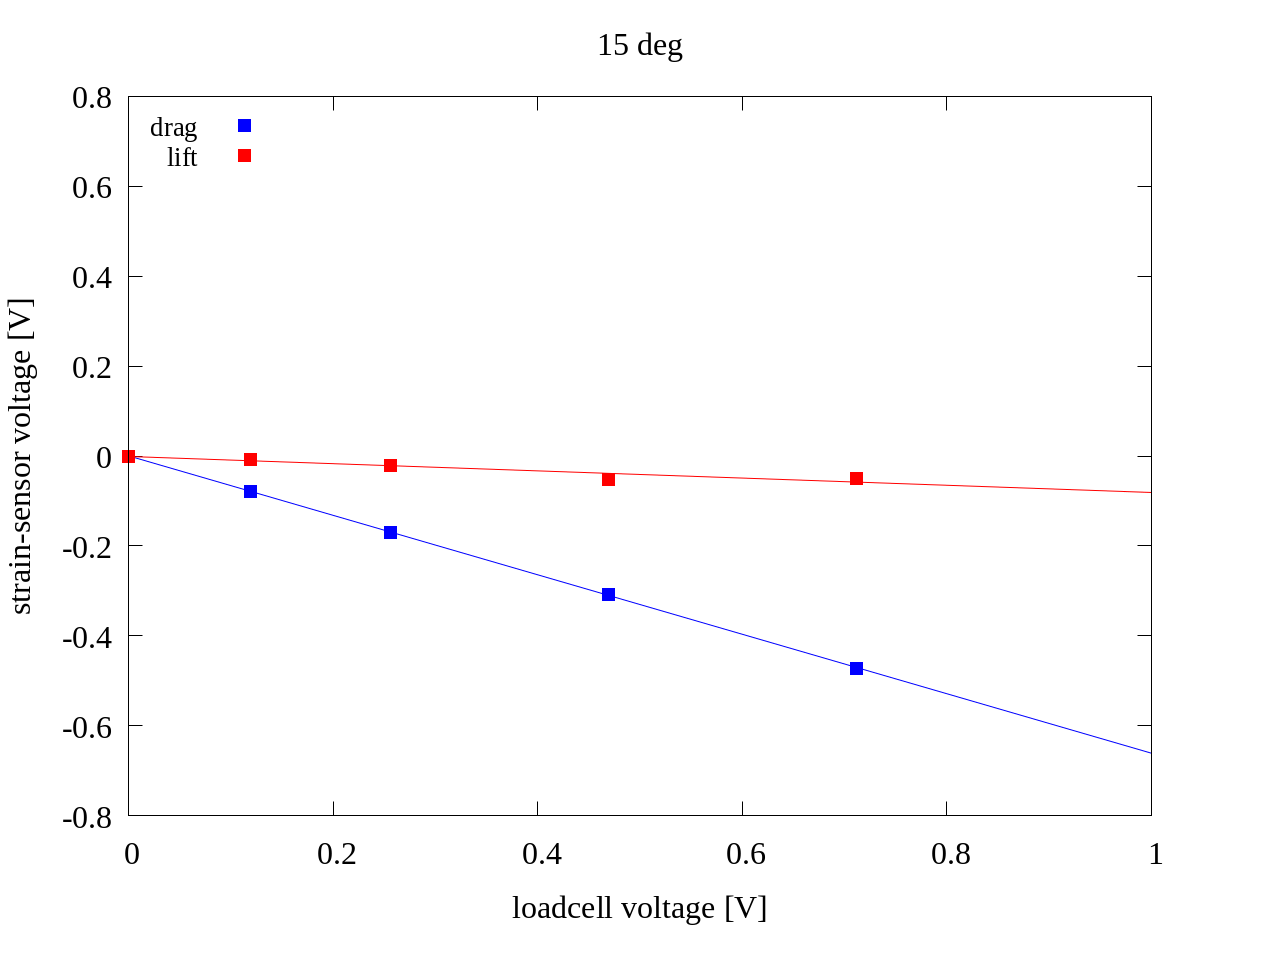
\includegraphics[width=78mm]{../images/linear/15_linear.png}
        \caption{Result of 15 deg}
        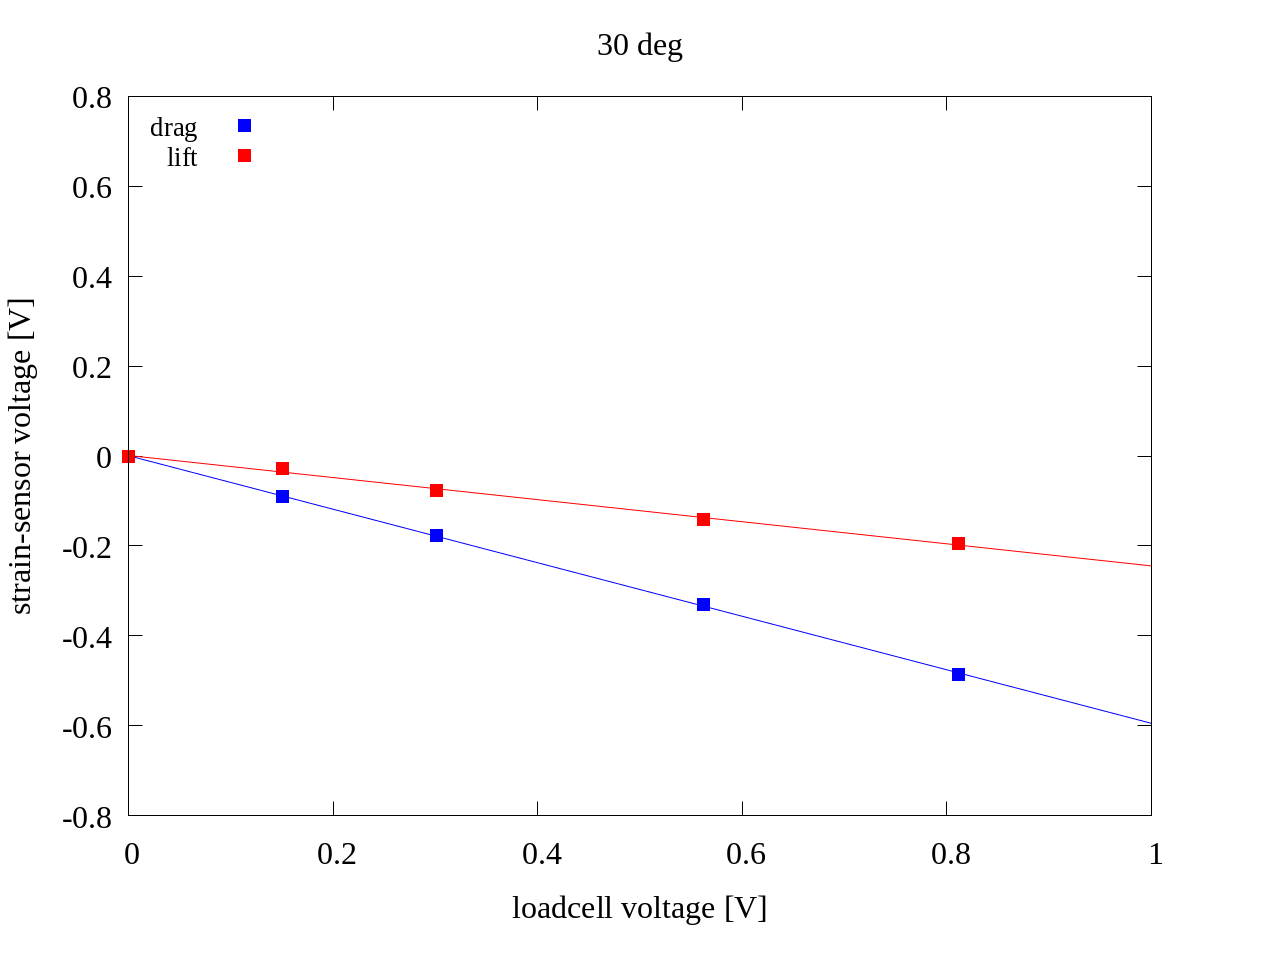
\includegraphics[width=78mm]{../images/linear/30_linear.png}
        \caption{Result of 30 deg}
    \end{center}
\end{figure}
\begin{figure}[htbp]
    \footnotesize
    \begin{center}
        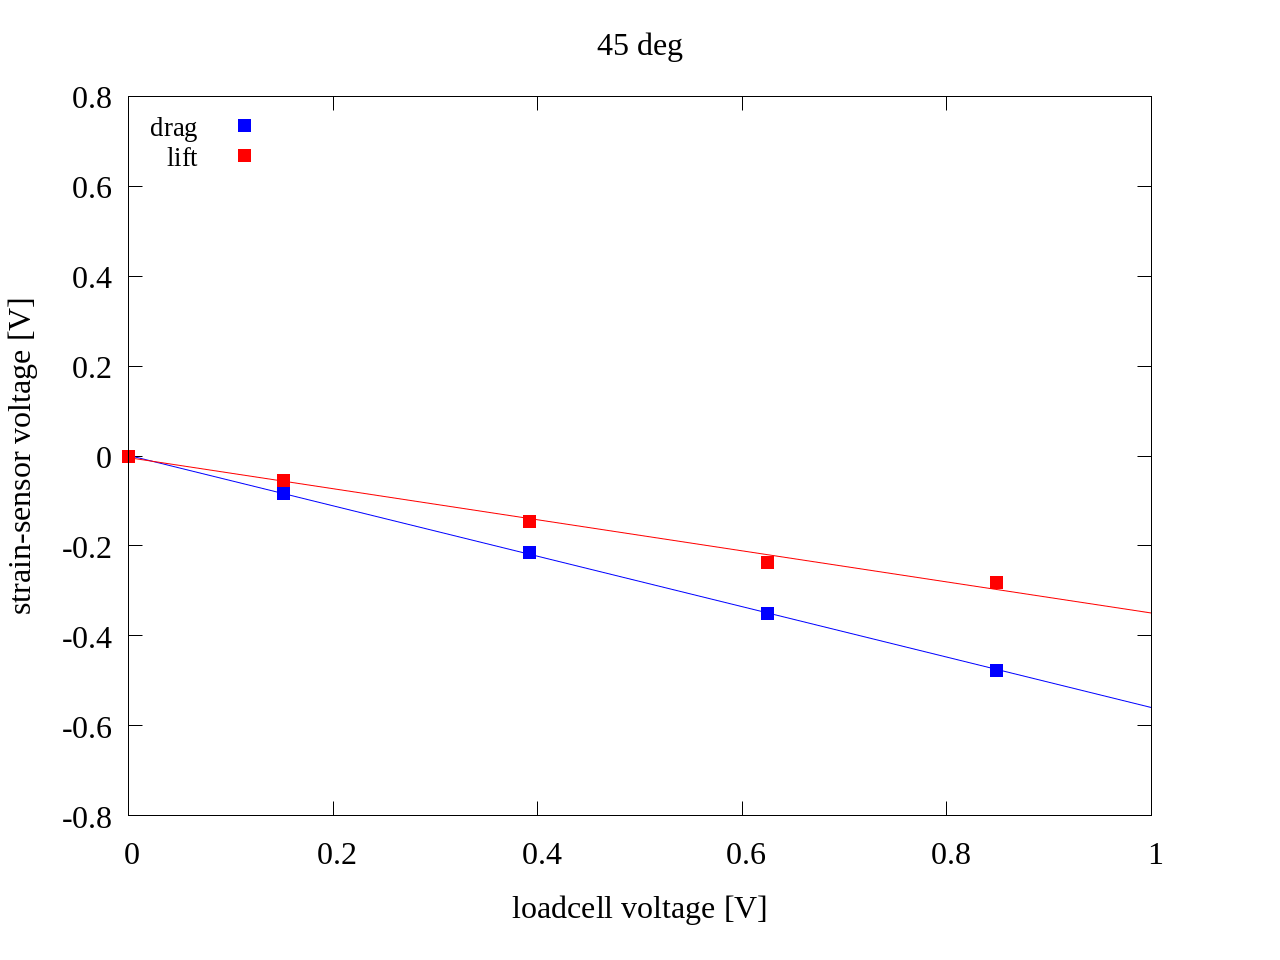
\includegraphics[width=78mm]{../images/linear/45_linear.png}
        \caption{Result of 45 deg}
        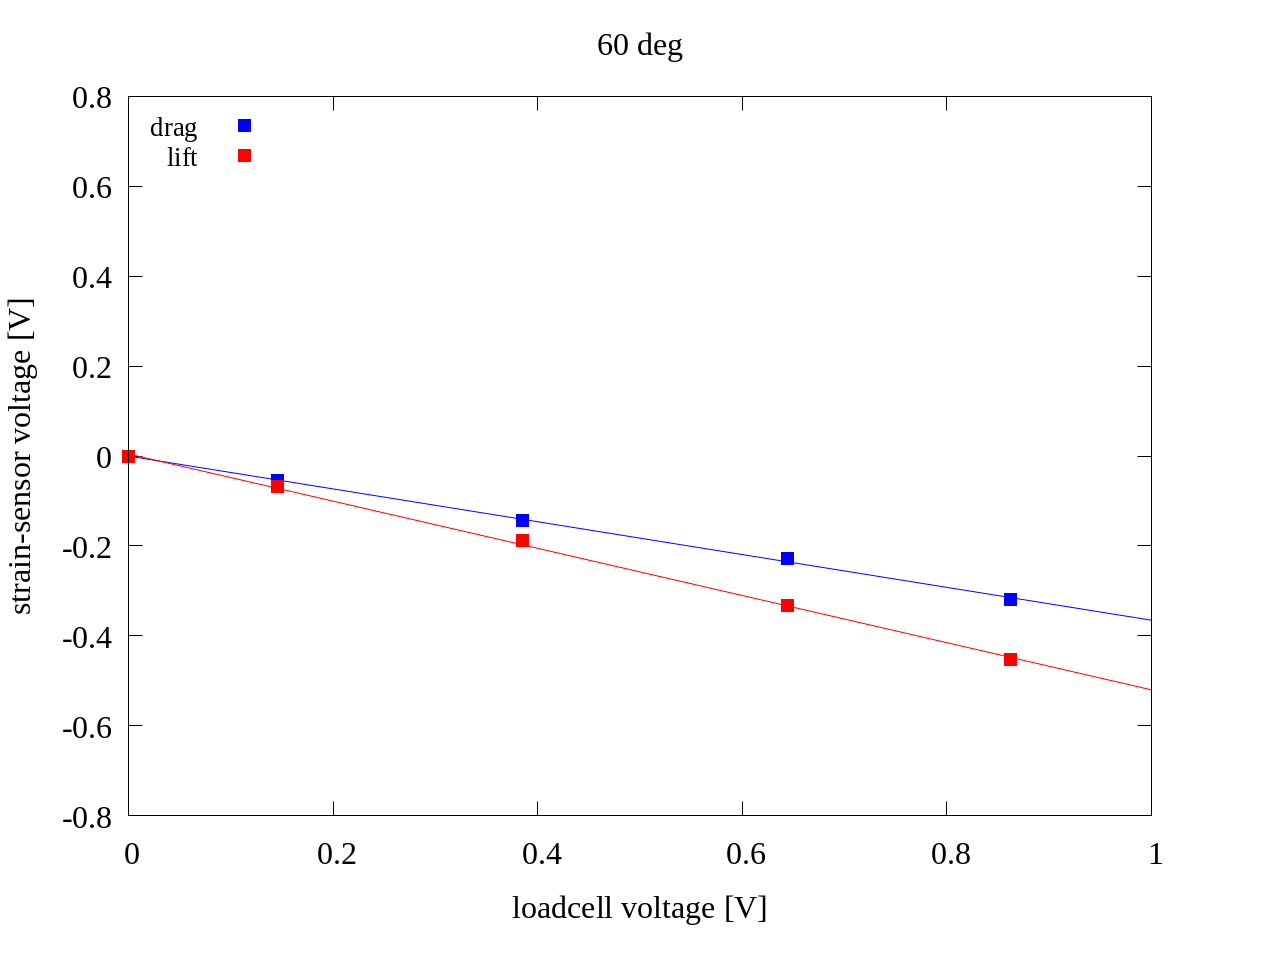
\includegraphics[width=78mm]{../images/linear/60_linear.png}
        \caption{Result of 60 deg}
        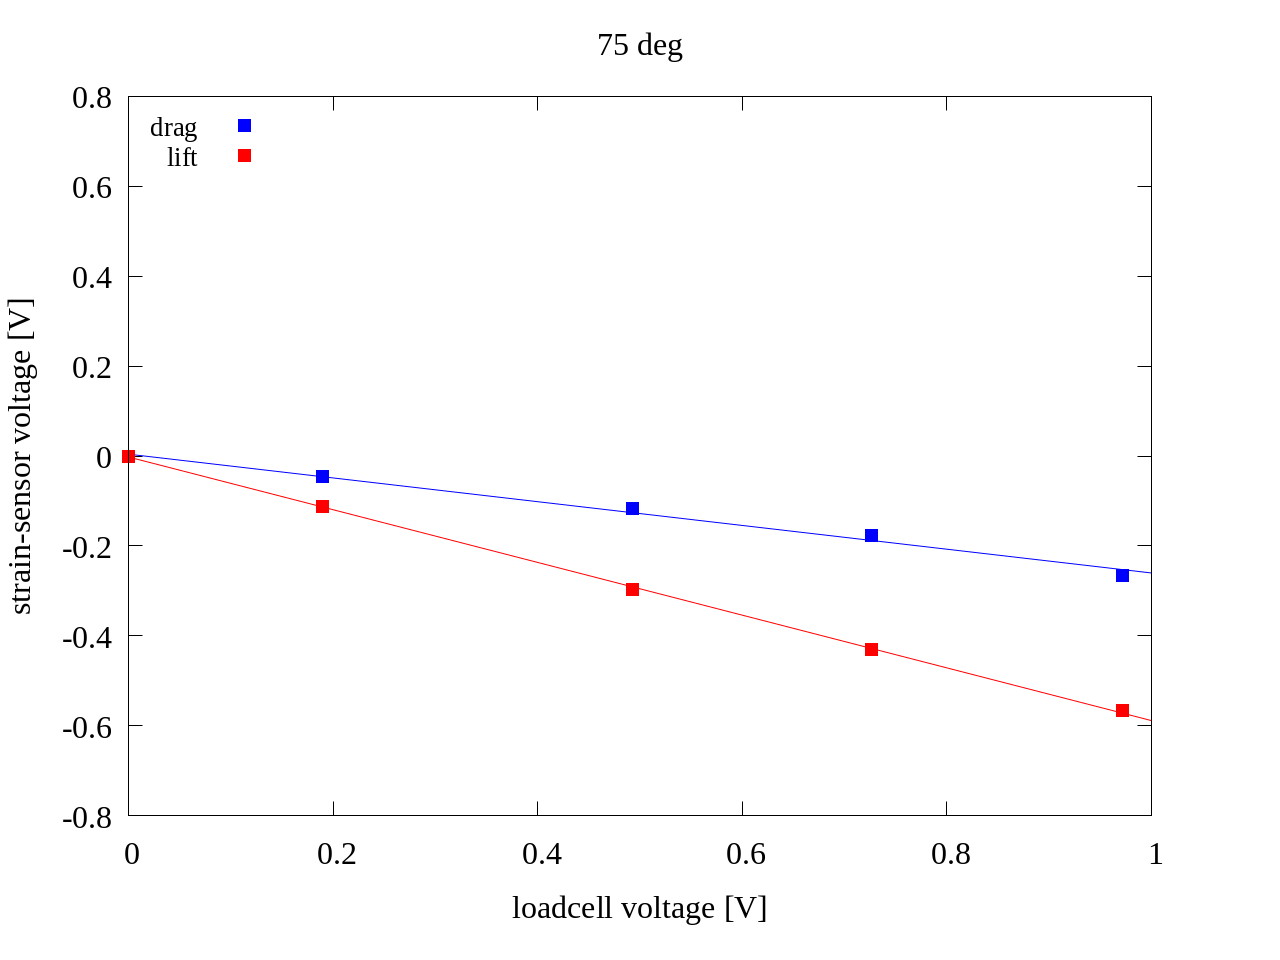
\includegraphics[width=78mm]{../images/linear/75_linear.png}
        \caption{Result of 75 deg}
        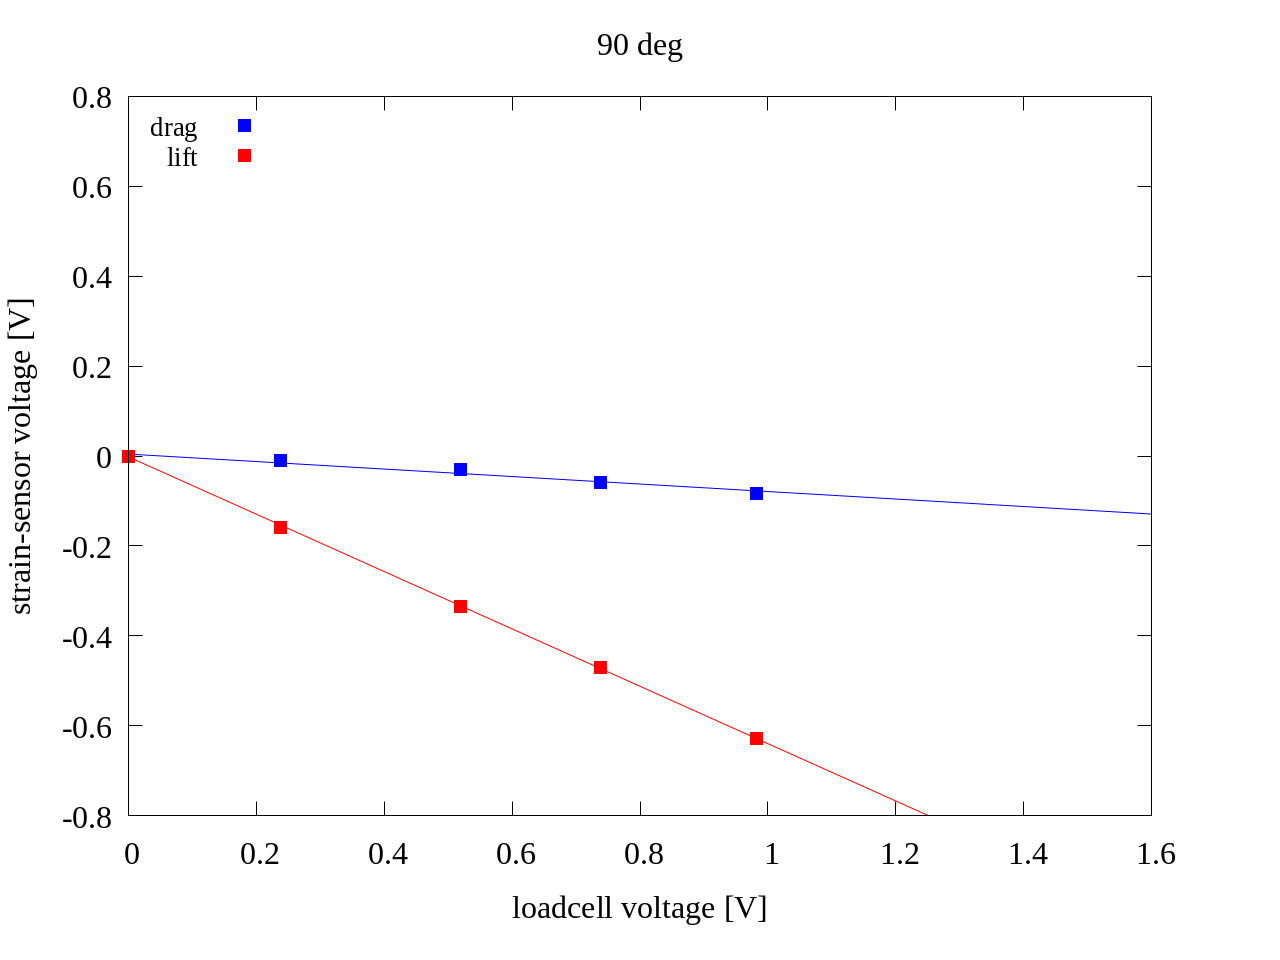
\includegraphics[width=78mm]{../images/linear/90_linear.png}
        \caption{Result of 90 deg}
    \end{center}
\end{figure}

\newpage
\subsection{二乗和平方根の算出}

取得したデータを用いて二乗和平方根の算出を行った.
その結果を以下のFig.16,Fig.17に示す.

\begin{table}[htbp]
    \begin{center}
        \begin{tabular}{|p{20mm}|p{20mm}|p{20mm}|p{20mm}|}
            \hline
            \multicolumn{1}{|c|}{\textgt{Angle [deg]}}  & \multicolumn{1}{|c|}{\textgt{Drag [V/V]}}  & \multicolumn{1}{|c|}{\textgt{Lift [V/V]}} & \multicolumn{1}{|c|}{\textgt{Sqrt [V/V]}}\\ \hline
            \multicolumn{1}{|c|}{0}                     & \multicolumn{1}{|c|}{-0.6484}              & \multicolumn{1}{|c|}{\textgt{0.0839}}     & \multicolumn{1}{|c|}{\textgt{0.6539}}\\ \hline
            \multicolumn{1}{|c|}{15}                    & \multicolumn{1}{|c|}{-0.6617}              & \multicolumn{1}{|c|}{\textgt{-0.0781}}    & \multicolumn{1}{|c|}{\textgt{0.6665}}\\ \hline
            \multicolumn{1}{|c|}{30}                    & \multicolumn{1}{|c|}{-0.5956}              & \multicolumn{1}{|c|}{\textgt{-0.2457}}    & \multicolumn{1}{|c|}{\textgt{0.6443}}\\ \hline
            \multicolumn{1}{|c|}{45}                    & \multicolumn{1}{|c|}{-0.5610}              & \multicolumn{1}{|c|}{\textgt{-0.3457}}    & \multicolumn{1}{|c|}{\textgt{0.6590}}\\ \hline
            \multicolumn{1}{|c|}{60}                    & \multicolumn{1}{|c|}{-0.3652}              & \multicolumn{1}{|c|}{\textgt{-0.5248}}    & \multicolumn{1}{|c|}{\textgt{0.6394}}\\ \hline
            \multicolumn{1}{|c|}{75}                    & \multicolumn{1}{|c|}{-0.2643}              & \multicolumn{1}{|c|}{\textgt{-0.5866}}    & \multicolumn{1}{|c|}{\textgt{0.6434}}\\ \hline
            \multicolumn{1}{|c|}{90}                    & \multicolumn{1}{|c|}{-0.0833}              & \multicolumn{1}{|c|}{\textgt{-0.6378}}    & \multicolumn{1}{|c|}{\textgt{0.6434}}\\ \hline
            \multicolumn{1}{|c|}{105}                   & \multicolumn{1}{|c|}{}              & \multicolumn{1}{|c|}{\textgt{}}    & \multicolumn{1}{|c|}{\textgt{}}\\ \hline
            \multicolumn{1}{|c|}{120}                   & \multicolumn{1}{|c|}{}              & \multicolumn{1}{|c|}{\textgt{}}    & \multicolumn{1}{|c|}{\textgt{}}\\ \hline
            \multicolumn{1}{|c|}{135}                   & \multicolumn{1}{|c|}{}              & \multicolumn{1}{|c|}{\textgt{}}    & \multicolumn{1}{|c|}{\textgt{}}\\ \hline
            \multicolumn{1}{|c|}{150}                   & \multicolumn{1}{|c|}{}              & \multicolumn{1}{|c|}{\textgt{}}    & \multicolumn{1}{|c|}{\textgt{}}\\ \hline
            \multicolumn{1}{|c|}{165}                   & \multicolumn{1}{|c|}{}              & \multicolumn{1}{|c|}{\textgt{}}    & \multicolumn{1}{|c|}{\textgt{}}\\ \hline
            \multicolumn{1}{|c|}{180}                   & \multicolumn{1}{|c|}{}              & \multicolumn{1}{|c|}{\textgt{}}    & \multicolumn{1}{|c|}{\textgt{}}\\ \hline
            \multicolumn{1}{|c|}{195}                   & \multicolumn{1}{|c|}{}              & \multicolumn{1}{|c|}{\textgt{}}    & \multicolumn{1}{|c|}{\textgt{}}\\ \hline
            \multicolumn{1}{|c|}{210}                   & \multicolumn{1}{|c|}{}              & \multicolumn{1}{|c|}{\textgt{}}    & \multicolumn{1}{|c|}{\textgt{}}\\ \hline
            \multicolumn{1}{|c|}{225}                   & \multicolumn{1}{|c|}{}              & \multicolumn{1}{|c|}{\textgt{}}    & \multicolumn{1}{|c|}{\textgt{}}\\ \hline
            \multicolumn{1}{|c|}{240}                   & \multicolumn{1}{|c|}{}              & \multicolumn{1}{|c|}{\textgt{}}    & \multicolumn{1}{|c|}{\textgt{}}\\ \hline
            \multicolumn{1}{|c|}{255}                   & \multicolumn{1}{|c|}{}              & \multicolumn{1}{|c|}{\textgt{}}    & \multicolumn{1}{|c|}{\textgt{}}\\ \hline
            \multicolumn{1}{|c|}{270}                   & \multicolumn{1}{|c|}{}              & \multicolumn{1}{|c|}{\textgt{}}    & \multicolumn{1}{|c|}{\textgt{}}\\ \hline
            \multicolumn{1}{|c|}{285}                   & \multicolumn{1}{|c|}{}              & \multicolumn{1}{|c|}{\textgt{}}    & \multicolumn{1}{|c|}{\textgt{}}\\ \hline
            \multicolumn{1}{|c|}{300}                   & \multicolumn{1}{|c|}{}              & \multicolumn{1}{|c|}{\textgt{}}    & \multicolumn{1}{|c|}{\textgt{}}\\ \hline
            \multicolumn{1}{|c|}{315}                   & \multicolumn{1}{|c|}{}              & \multicolumn{1}{|c|}{\textgt{}}    & \multicolumn{1}{|c|}{\textgt{}}\\ \hline
            \multicolumn{1}{|c|}{330}                   & \multicolumn{1}{|c|}{}              & \multicolumn{1}{|c|}{\textgt{}}    & \multicolumn{1}{|c|}{\textgt{}}\\ \hline
            \multicolumn{1}{|c|}{345}                   & \multicolumn{1}{|c|}{}              & \multicolumn{1}{|c|}{\textgt{}}    & \multicolumn{1}{|c|}{\textgt{}}\\ \hline
        \end{tabular}
    \end{center}
\end{table}

\begin{figure}[htbp]
    \footnotesize
    \begin{center}
        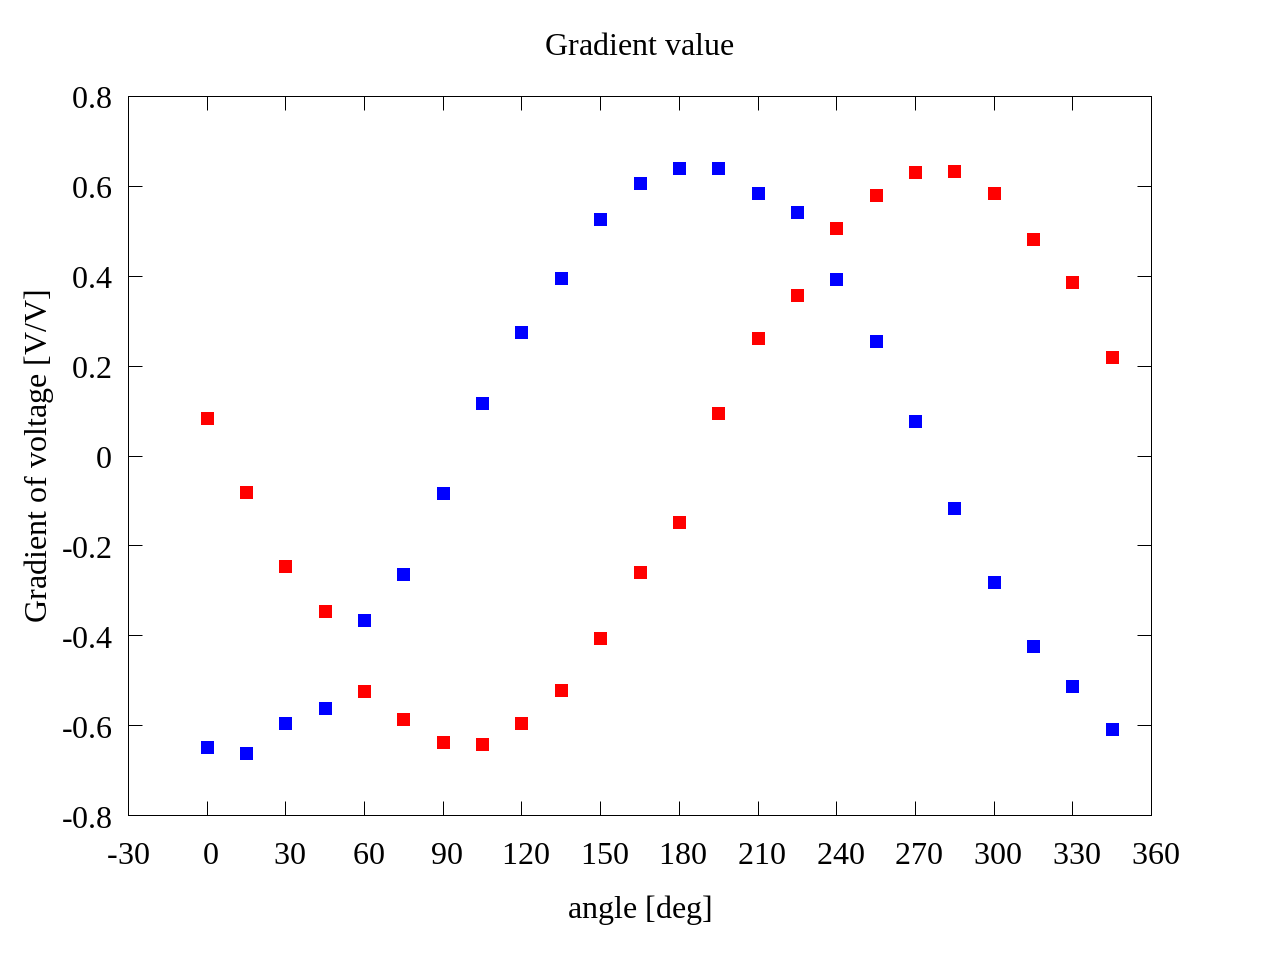
\includegraphics[width=85mm]{../images/summary/summary_1.png}
        \caption{Summary of gradient value}
        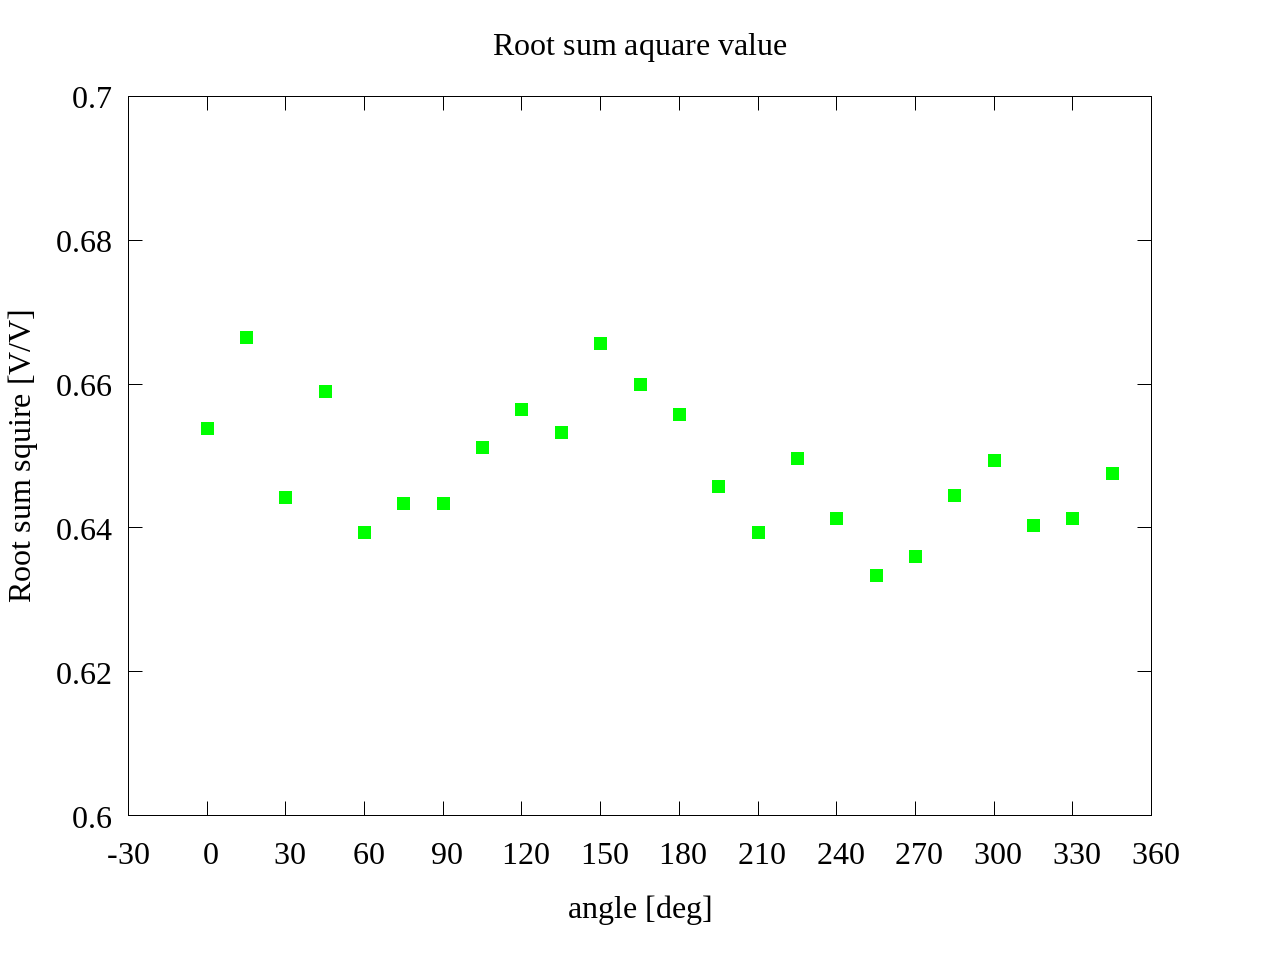
\includegraphics[width=85mm]{../images/summary/summary_2.png}
        \caption{Summary of root sum square value}
    \end{center}
\end{figure}

\end{document}